\documentclass{beamer}
\usetheme{Madrid}

%packages
\usepackage{graphicx}
\usepackage{tikz}

%graphics
\graphicspath{img}

\title{Inferring community characteristics in labelled networks}
\subtitle{IIB Project}
\author{Lawrence Tray}
\institute{Ioannis Kontoyiannis}
\date{\today}

\begin{document}
	
	\begin{frame}
		\titlepage
	\end{frame}

	\begin{frame}{Motivation}

	\end{frame}

	\begin{frame}{The feature-first block model (FFBM)}
		\begin{figure}[!h]
			\centering
			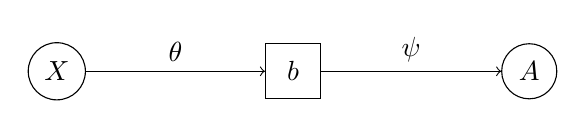
\begin{tikzpicture}[
				roundnode/.style={circle, draw=black, minimum size=7mm},
				squarednode/.style={rectangle, draw=black, minimum size=7mm}
				]
				% nodes
				\node[roundnode] (X) at (0, 0) {$X$};
				\node[squarednode] (b) at (3, 0) {$b$};
				\node[roundnode] (A) at (6, 0) {$A$};
				
				% arrows
				\draw[->] (X.east) -- node[above] {$\theta$} (b.west);
				\draw[->] (b.east) -- node[above] {$\psi$}(A.west);
			\end{tikzpicture}
			\caption{The feature-first block model (FFBM)}
			\label{fig:ffbm}
		\end{figure}
	
		\begin{align}
			p(b|X; \theta) &= \prod_{i \in [N]} \phi_{b_i} (x_i; \theta)
			= \prod_{i \in [N]} \frac{\exp (w_{b_i}^T x_i)}{\sum_{k \in [B]} \exp (w_k^T x_i) } \\ \nonumber \\
			p(A|b; \psi) &\sim \textrm{DC-SBM}_{\textrm{MC}} (b, \psi_e, \psi_k)
		\end{align}
	\end{frame}

	\begin{frame}{Inference procedure}
		We want to draw:
		\begin{equation}
			\theta^{(t)} \sim p(\theta| A, X).
		\end{equation}
		We achieve this by:
		\begin{align}
			b^{(t)} &\sim p \Big( b| A, X \Big) \\
			\theta^{(t)} &\sim p \Big( \theta| X, b^{(t)} \Big)
		\end{align}
	\end{frame}
	
	\begin{frame}{Sampling sequence}
		\begin{figure}[!h]
			\centering
			
			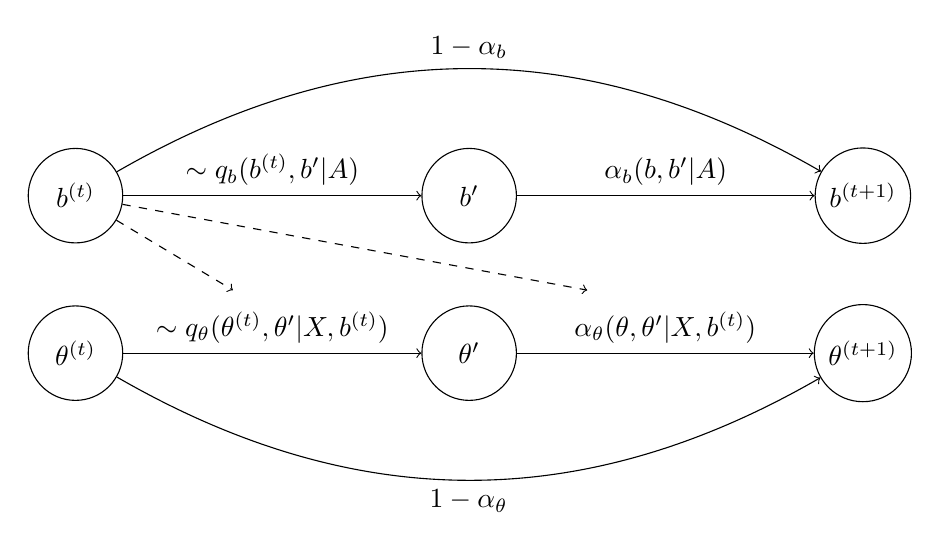
\begin{tikzpicture}[
				roundnode/.style={circle, draw=black, minimum size=12mm},
				squarednode/.style={rectangle, draw=black, minimum size=12mm}
				]
				% nodes
				\node[roundnode] (b0) at (0, 2) {$b^{(t)}$};
				\node[roundnode] (b1) at (5, 2) {$b'$};
				\node[roundnode] (b2) at (10, 2) {$b^{(t+1)}$};
				\node[roundnode] (t0) at (0, 0) {$\theta^{(t)}$};
				\node[roundnode] (t1) at (5, 0) {$\theta'$};
				\node[roundnode] (t2) at (10, 0) {$\theta^{(t+1)}$};
				
				% arrows
				\draw[->] (b0) to node[above] {$\sim q_b(b^{(t)}, b' | A)$} (b1);
				\draw[->] (b1) to node[above] {$\alpha_b (b, b' | A)$} (b2);
				\draw[->] (b0) [out=30, in=150] to node[above] {$1-\alpha_b$} (b2);
				
				\draw[->] (t0) to node[above] {$\sim q_\theta(\theta^{(t)}, \theta' | X, b^{(t)})$} (t1);
				\draw[->] (t1) to node[above] {$\alpha_\theta (\theta, \theta' | X, b^{(t)})$} (t2);
				\draw[->] (t0) [out=-30, in=-150] to node[below] {$1-\alpha_\theta$} (t2);
				
				\draw[dashed, ->] (b0) to (2, 0.8);
				\draw[dashed, ->] (b0) to (6.5, 0.8);
				
			\end{tikzpicture}
			\caption{Sampling sequence.}
			\label{fig:samp-sequence}
		\end{figure}
	\end{frame}

\end{document}
